%%%%%%%%%%%%%%%%%%%%%%%%%%%%%%%%%%%%%%%%%
% fphw Assignment
% LaTeX Template
% Version 1.0 (27/04/2019)
%
% This template originates from:
% https://www.LaTeXTemplates.com
%
% Authors:
% Class by Felipe Portales-Oliva (f.portales.oliva@gmail.com) with template 
% content and modifications by Vel (vel@LaTeXTemplates.com)
%
% Template (this file) License:
% CC BY-NC-SA 3.0 (http://creativecommons.org/licenses/by-nc-sa/3.0/)
%
%%%%%%%%%%%%%%%%%%%%%%%%%%%%%%%%%%%%%%%%%

%----------------------------------------------------------------------------------------
%	PACKAGES AND OTHER DOCUMENT CONFIGURATIONS
%----------------------------------------------------------------------------------------

\documentclass[
	12pt, % Default font size, values between 10pt-12pt are allowed
	%letterpaper, % Uncomment for US letter paper size
	%spanish, % Uncomment for Spanish
]{fphw}

% Template-specific packages
\usepackage[utf8]{inputenc} % Required for inputting international characters
\usepackage[T1]{fontenc} % Output font encoding for international characters
\usepackage{mathpazo} % Use the Palatino font

\usepackage{graphicx} % Required for including images

\usepackage{booktabs} % Required for better horizontal rules in tables

\usepackage{listings, listings-rust} % Required for insertion of code

\usepackage{enumerate} % To modify the enumerate environment

%----------------------------------------------------------------------------------------
%	ASSIGNMENT INFORMATION
%----------------------------------------------------------------------------------------

\title{Assignment \#2: Building the Symbol Table Stack} % Assignment title


\date{DUE DATE} % Due date

\institute{Union College} % Institute or school name

\class{CSC-375 Compiler Design} % Course or class name

\professor{Aaron Cass} % Professor or teacher in charge of the assignment

%----------------------------------------------------------------------------------------

\begin{document}

\maketitle % Output the assignment title, created automatically using the information in the custom commands above

%----------------------------------------------------------------------------------------
%	ASSIGNMENT CONTENT
%----------------------------------------------------------------------------------------

\section*{Objectives}

\begin{problem}
	\begin{itemize}
	    \item Deepen your understanding of the Rust programming language
        \item Learn how to construct and manage symbol tables in a compiler
        \item Thoroughly test the Symbol Table Stack to assure functionality
	\end{itemize}
\end{problem}

%------------------------------------------------

\subsection*{An explanation of symbol tables:}
In compiler design, a symbol table is a data structure used by a compiler to keep track of scope and binding information about names. Symbol tables are essential for semantic analysis, which checks for correct use of variables, functions, classes, and other entities. They allow the compiler to quickly verify and retrieve information about these entities, facilitating tasks such as type checking, memory allocation, and scope resolution. In this assignment, you will build the structure to manage a stack of symbol tables, representing different levels of scope within a program.

\begin{figure}[h!]
    \centering
    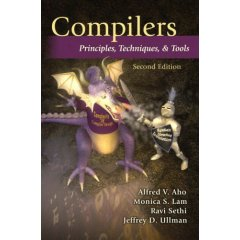
\includegraphics[width=0.5\textwidth]{dragon.jpeg}
    \caption{A more comprehensive explanation of the symbol table and the symbol table stack can be found in sections 1.2.7 (page 11) and 2.7 (page 85) of the dragon book.}
    \label{fig:symbol_table_structure}
\end{figure}
\pagebreak
%----------------------------------------------------------------------------------------

\section*{Symbol Table Stack Structure}

\lstinputlisting[
    caption=mod.rs, % Caption above the listing
    label=lst:modsymtab, % Label for referencing this listing
    language=Rust, % Use Rust functions/syntax highlighting
    frame=single, % Frame around the code listing
    showstringspaces=false, % Don't put marks in string spaces
    numbers=left, % Line numbers on left
    numberstyle=\tiny, % Line numbers styling
]

\section*{lib.rs:}
This file defines the modules related to the symbol table stack and makes them available for other modules to see. It can be found in the \textit{frontend/} folder. All modules each have documentation in this file to show what the module is used for. The symbol table stack involves several submodules: the symbol table, symbol info, and the stack itself.\\
\\
You don't have to do anything to this file.

\section*{core.rs:}
This file contains the core logic for generating the symbol table stack and routing AST nodes to appropriate handlers. While the structure for \textbf{SymbolValue, SymbolInfo, SymbolTable, and SymbolTableStack} are given, additional functions for utilizing these struct's and enum's will need to be implemented. You will also need to implement the following core functions:
\begin{itemize}
    \item \textbf{gen\_sym\_table\_stack}: Drives the symbol table stack generation process and returns the original AST and the generated symbol table stack, or errors if any.
    \item \textbf{sym\_table\_stack\_router}: Routes the proper top-level expression for an ASTNode.
\end{itemize}

\section*{block.rs:}
This file contains the implementation of block statements (e.g., functions, loops) within the symbol table stack. You will need to implement the following functions:
\begin{itemize}
    \item \textbf{sym\_table\_fn}: Adds a function type to the current scope.
    \item \textbf{sym\_table\_struct}: Adds a struct type to the current scope.
    \item \textbf{sym\_table\_enum}: Adds an enum type to the current scope.
    \item \textbf{sym\_table\_while}: Adds a while loop to the current scope.
    \item \textbf{sym\_table\_do\_while}: Adds a do-while loop to the current scope.
    \item \textbf{sym\_table\_for}: Adds a for loop to the current scope.
    \item \textbf{sym\_table\_if\_else}: Adds an if-else block to the current scope.
    \item \textbf{sym\_table\_switch}: Adds a switch statement to the current scope.
\end{itemize}
\pagebreak
\section*{statement.rs:}
This file contains functions that define statements and variables within blocks. The following functions need to be implemented:
\begin{itemize}
    \item \textbf{sym\_table\_init}: Adds a new variable into the current scope.
    \item \textbf{sym\_table\_assign}: Assigns a new value to a variable in the current scope.
\end{itemize}

\section*{base\_tests.rs:}
This file contains test definitions for base case tests. Your job is to implement and expand upon these tests to assure proper scope management. 

\section*{combination\_tests.rs:}
This file should be used as a test suite for combination tests of elements tested in \textbf{base\_tests.rs}. Make sure to comprehensively test these combinations. 

\section*{edge\_tests.rs:}
This file should be used as a test suite for boundary cases. This suite should comprehensively test the addition and functionality of SyntaxElements within the Symbol Table Stack. 

\section*{error\_tests.rs:}
This file should be used as a test suite for error handling. Comprehensively test that every instance that may raise an error is handled properly. 

\pagebreak

\section*{Follow these guidelines to build the symbol table stack}

\begin{problem}
    \begin{enumerate}
        \item Do not change any of the function signatures, i.e., leave all parameters, parameter types, and return types as you found them.
        \item Follow all instructions given in the comments where they exist, and take any potential hints into consideration when making your design.
        \item Remember you are managing a stack of symbol tables, each representing a different scope. Ensure that your implementation correctly handles scope transitions.
        \item Use the \textbf{SymbolInfo}, \textbf{SymbolTable}, and \textbf{SymbolTableStack} structs effectively to maintain the integrity of the symbol table stack.
        \item Maintain clear and consistent error handling. Use \textbf{Result} and \textbf{ErrorType} to propagate errors appropriately.
    \end{enumerate}
\end{problem}

\section*{Cheat sheet for manipulating symbol tables}

\begin{problem}
    It might not be obvious how to manipulate symbol tables effectively. Here are some tips on how to do this.
    \\
    \begin{enumerate}
        \item When adding a new symbol to a table, ensure you use the \textbf{add} method of \textbf{SymbolTable}. For example, if you want to add a function, create a \textbf{SymbolInfo} object and use \textbf{SymbolTable::add}.
        \item When transitioning scopes, use the \textbf{push} and \textbf{pop} methods of \textbf{SymbolTableStack} to manage the stack of tables. For example, when entering a new scope, push a new table onto the stack.
        \item To retrieve symbols from the current scope, use the \textbf{get} method of \textbf{SymbolTable}. Ensure you handle cases where the symbol might not be found.
        \item Maintain clear and consistent error handling. Use \textbf{Result} and \textbf{ErrorType} to propagate errors appropriately.
    \end{enumerate}
\end{problem}

\pagebreak

\end{document}
